\documentclass[tikz]{standalone}

\usetikzlibrary{arrows,positioning}

\begin{document}
	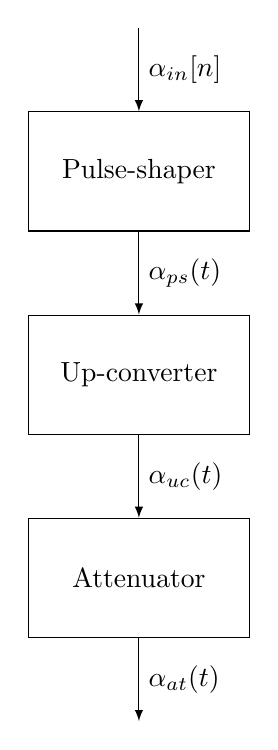
\begin{tikzpicture}[
		node distance=3em,
		arrow/.style={-latex},
		block/.style={draw, minimum height=10ex, minimum width=8em, align=center},
	]
		\coordinate (in) at (0,0);
		\node (ps) [block, below=of in] {Pulse-shaper};
		\node (uc) [block, below=of ps] {Up-converter};
		\node (at) [block, below=of uc] {Attenuator};
		\coordinate[below=of at] (out);
		
		\draw[arrow] (in) -- node[anchor=west]{$\alpha_\text{in}[n]$} (ps);
		\draw[arrow] (ps) -- node[anchor=west]{$\alpha_\text{ps}(t)$} (uc);
		\draw[arrow] (uc) -- node[anchor=west]{$\alpha_\text{uc}(t)$} (at);
		\draw[arrow] (at) -- node[anchor=west]{$\alpha_\text{at}(t)$} (out);
	\end{tikzpicture}
\end{document}
